\RequirePackage{fix-cm}
\documentclass[smallextended,epjc3]{svjour3}
\smartqed

\usepackage[T1]{fontenc}
\usepackage[utf8]{inputenc}
\usepackage[a4paper,textwidth=17.4cm,textheight=248mm,centering]{geometry}
\usepackage{microtype}
\usepackage{amsmath,amssymb,booktabs,longtable,array,graphicx,xcolor}
\usepackage[hyphens]{url}
\usepackage[hidelinks]{hyperref}
\graphicspath{{editorial_figures/}{./}}
\Urlmuskip=0mu plus 2mu\relax
\setlength{\emergencystretch}{2.5em}
\raggedbottom

\makeatletter
\def\institute@and{\par\noindent\institute@mark}
\g@addto@macro\@evenhead{\hfil}
\def\LT@makecaption#1#2#3{%
  \LT@mcol\LT@cols c{\hbox to\z@{\hss\parbox[t]\LTcapwidth{%
    \normalfont\small
    \sbox\@tempboxa{#1{{\bfseries #2\enspace}}#3}%
    \ifdim\wd\@tempboxa>\hsize
      #1{{\bfseries #2\enspace}}#3\par
    \else
      \hbox to\hsize{\unhbox\@tempboxa\hfil}%
    \fi
    \vskip5.5pt}%
  \hss}}}
\makeatother

\journalname{Eur. Phys. J. C}

\newcommand{\pin}{p_{\mathrm{in}}}
\newcommand{\pout}{p_{\mathrm{out}}}
\newcommand{\deltap}{\Delta p}
\newcommand{\phys}{\mathrm{BB}}
\newcommand{\raw}{\mathrm{Raw}}
\newcommand{\learned}{\mathrm{PR}}
\newcommand{\simple}{\mathrm{Lin}}

\renewcommand{\thesection}{S\arabic{section}}
\renewcommand{\thetable}{S\arabic{table}}
\renewcommand{\thefigure}{S\arabic{figure}}
\renewcommand{\theequation}{S\arabic{equation}}

\begin{document}
\setlength{\LTcapwidth}{\textwidth}

\title{Electronic Supplementary Material:\\Non-monotonic benefits of physical target centering in conditional models of pion momentum loss}
\titlerunning{Supplementary Material: Physical target centering in pion momentum loss}

\author{Xuansong Chang\thanksref{e1,addr1} \and
        Yiran Xiao\thanksref{addr1} \and
        Chengtao Song\thanksref{addr2}}
\authorrunning{X. Chang et al.}

\thankstext{e1}{e-mail: \href{mailto:alec.xs.chang@gmail.com}{alec.xs.chang@gmail.com}}

\institute{Anhui University, Hefei, China\label{addr1}
           \and
           Xi'an Jiaotong University, Xi'an, China\label{addr2}}

\date{Received: date / Accepted: date}

\maketitle

Current C/D evidence precedes numerical and reproduction details. Display
names map to frozen identifiers in Sect.~\ref{sec:display_mapping}; the
standalone historical archive retains earlier A/B and erroneous-center evidence.

\section{Complete primary C/D results}
\label{sec:primary}

Symbols $N$, $M_2$, $M_8$ and $E$ denote no direct, two-bin, eight-bin and
exact momentum inputs. Event intervals condition on selected models; seed
spreads describe shared-data optimizer variability.

\begin{table}[!htbp]
\centering
\normalsize
\setlength{\tabcolsep}{3pt}
\caption{All 16 prespecified contrasts on catalog C (499,285 eligible events). $\Delta$ is mean Raw-minus-BB-centered NLL across five paired optimizer seeds; differences are more minus less information. Intervals are approximate 95\% simultaneous event-bootstrap intervals within this catalog (2000 resamples), conditional on fixed models. Seed SD describes optimizer variation, not interval uncertainty; $n_+$ counts positive seeds. Units: nat per eligible event.}
\label{tab:information-C-primary16}
\begin{tabular}{llrrrrr}
\toprule
Contrast & Train & Mean & Seed SD & 95\% lower & 95\% upper & $n_+/5$ \\
\midrule
$\Delta_{\mathrm{N}}$ & 10\% & $+0.006272$ & $0.000811$ & $+0.005709$ & $+0.006835$ & 5/5 \\
$\Delta_{\mathrm{M_2}}$ & 10\% & $+0.010399$ & $0.001099$ & $+0.009844$ & $+0.010954$ & 5/5 \\
$\Delta_{\mathrm{M_8}}$ & 10\% & $+0.003082$ & $0.001596$ & $+0.002741$ & $+0.003423$ & 5/5 \\
$\Delta_{\mathrm{E}}$ & 10\% & $+0.001845$ & $0.001855$ & $+0.001580$ & $+0.002110$ & 4/5 \\
\midrule
$\Delta_{\mathrm{N}}$ & 100\% & $+0.006233$ & $0.001125$ & $+0.005661$ & $+0.006804$ & 5/5 \\
$\Delta_{\mathrm{M_2}}$ & 100\% & $+0.010895$ & $0.001060$ & $+0.010287$ & $+0.011502$ & 5/5 \\
$\Delta_{\mathrm{M_8}}$ & 100\% & $+0.002987$ & $0.001211$ & $+0.002653$ & $+0.003321$ & 5/5 \\
$\Delta_{\mathrm{E}}$ & 100\% & $+0.001550$ & $0.000923$ & $+0.001300$ & $+0.001799$ & 5/5 \\
\midrule
$\Delta_{\mathrm{M_2}}-\Delta_{\mathrm{N}}$ & 10\% & $+0.004127$ & $0.000767$ & $+0.003838$ & $+0.004417$ & 5/5 \\
$\Delta_{\mathrm{M_8}}-\Delta_{\mathrm{M_2}}$ & 10\% & $-0.007317$ & $0.002210$ & $-0.007780$ & $-0.006854$ & 0/5 \\
$\Delta_{\mathrm{E}}-\Delta_{\mathrm{M_8}}$ & 10\% & $-0.001237$ & $0.002137$ & $-0.001496$ & $-0.000978$ & 1/5 \\
$\Delta_{\mathrm{E}}-\Delta_{\mathrm{N}}$ & 10\% & $-0.004427$ & $0.001796$ & $-0.004975$ & $-0.003879$ & 0/5 \\
\midrule
$\Delta_{\mathrm{M_2}}-\Delta_{\mathrm{N}}$ & 100\% & $+0.004662$ & $0.000809$ & $+0.004395$ & $+0.004929$ & 5/5 \\
$\Delta_{\mathrm{M_8}}-\Delta_{\mathrm{M_2}}$ & 100\% & $-0.007908$ & $0.000441$ & $-0.008447$ & $-0.007368$ & 0/5 \\
$\Delta_{\mathrm{E}}-\Delta_{\mathrm{M_8}}$ & 100\% & $-0.001437$ & $0.000673$ & $-0.001656$ & $-0.001219$ & 0/5 \\
$\Delta_{\mathrm{E}}-\Delta_{\mathrm{N}}$ & 100\% & $-0.004683$ & $0.001226$ & $-0.005204$ & $-0.004162$ & 0/5 \\
\bottomrule
\end{tabular}
\end{table}

\begin{table}[!htbp]
\centering
\normalsize
\setlength{\tabcolsep}{3pt}
\caption{All 16 prespecified contrasts on catalog D (499,275 eligible events). $\Delta$ is mean Raw-minus-BB-centered NLL across five paired optimizer seeds; differences are more minus less information. Intervals are approximate 95\% simultaneous event-bootstrap intervals within this catalog (2000 resamples), conditional on fixed models. Seed SD describes optimizer variation, not interval uncertainty; $n_+$ counts positive seeds. Units: nat per eligible event.}
\label{tab:information-D-primary16}
\begin{tabular}{llrrrrr}
\toprule
Contrast & Train & Mean & Seed SD & 95\% lower & 95\% upper & $n_+/5$ \\
\midrule
$\Delta_{\mathrm{N}}$ & 10\% & $+0.006401$ & $0.000778$ & $+0.005830$ & $+0.006971$ & 5/5 \\
$\Delta_{\mathrm{M_2}}$ & 10\% & $+0.010623$ & $0.001277$ & $+0.010059$ & $+0.011186$ & 5/5 \\
$\Delta_{\mathrm{M_8}}$ & 10\% & $+0.003320$ & $0.001609$ & $+0.002979$ & $+0.003662$ & 5/5 \\
$\Delta_{\mathrm{E}}$ & 10\% & $+0.001876$ & $0.001836$ & $+0.001609$ & $+0.002142$ & 4/5 \\
\midrule
$\Delta_{\mathrm{N}}$ & 100\% & $+0.006543$ & $0.001194$ & $+0.005962$ & $+0.007124$ & 5/5 \\
$\Delta_{\mathrm{M_2}}$ & 100\% & $+0.011196$ & $0.001030$ & $+0.010576$ & $+0.011816$ & 5/5 \\
$\Delta_{\mathrm{M_8}}$ & 100\% & $+0.003332$ & $0.001181$ & $+0.002989$ & $+0.003676$ & 5/5 \\
$\Delta_{\mathrm{E}}$ & 100\% & $+0.001659$ & $0.000973$ & $+0.001408$ & $+0.001911$ & 5/5 \\
\midrule
$\Delta_{\mathrm{M_2}}-\Delta_{\mathrm{N}}$ & 10\% & $+0.004222$ & $0.001046$ & $+0.003922$ & $+0.004522$ & 5/5 \\
$\Delta_{\mathrm{M_8}}-\Delta_{\mathrm{M_2}}$ & 10\% & $-0.007302$ & $0.002233$ & $-0.007776$ & $-0.006828$ & 0/5 \\
$\Delta_{\mathrm{E}}-\Delta_{\mathrm{M_8}}$ & 10\% & $-0.001445$ & $0.002087$ & $-0.001707$ & $-0.001182$ & 1/5 \\
$\Delta_{\mathrm{E}}-\Delta_{\mathrm{N}}$ & 10\% & $-0.004525$ & $0.001713$ & $-0.005084$ & $-0.003966$ & 0/5 \\
\midrule
$\Delta_{\mathrm{M_2}}-\Delta_{\mathrm{N}}$ & 100\% & $+0.004653$ & $0.000837$ & $+0.004386$ & $+0.004920$ & 5/5 \\
$\Delta_{\mathrm{M_8}}-\Delta_{\mathrm{M_2}}$ & 100\% & $-0.007864$ & $0.000526$ & $-0.008417$ & $-0.007310$ & 0/5 \\
$\Delta_{\mathrm{E}}-\Delta_{\mathrm{M_8}}$ & 100\% & $-0.001673$ & $0.000805$ & $-0.001901$ & $-0.001445$ & 0/5 \\
$\Delta_{\mathrm{E}}-\Delta_{\mathrm{N}}$ & 100\% & $-0.004884$ & $0.001447$ & $-0.005415$ & $-0.004352$ & 0/5 \\
\bottomrule
\end{tabular}
\end{table}


\clearpage
\begin{figure}[!htbp]
\centering
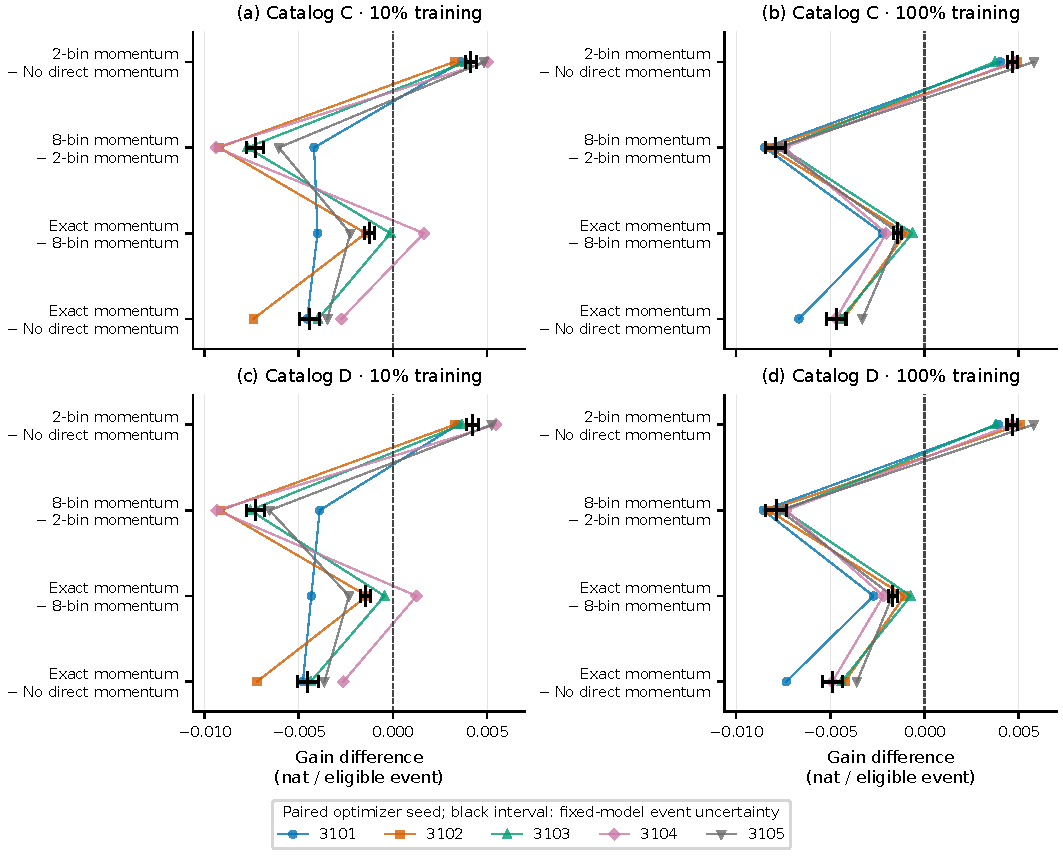
\includegraphics[width=0.92\linewidth]{information_gain_changes.pdf}
\caption{All adjacent and endpoint gain differences. Positive values mean
the more-informed conditioner has a larger centering gain. Black bands use
the 16-contrast simultaneous family within each catalog; all five paired
seed values remain visible.}
\label{fig:supp_gain_changes}
\end{figure}
\clearpage

\section{Training variability and conditional diagnostics}
\label{sec:diagnostics}

\subsection{Optimizer-seed sensitivity}
The sensitivity analysis was added after the C/D evaluation and does not
alter the frozen primary event-bootstrap family. Tables~\ref{tab:seed_sensitivity_C}
and \ref{tab:seed_sensitivity_D} retain every primary
contrast's mean, sample SD, range and sign counts, with each individual
paired seed value in the associated aggregate records.
The range of leave-one-seed-out means is a sensitivity summary, not a
confidence interval. C and D evaluate the same five models in each setting.

% Generated post-hoc to known C/D outcomes. Do not edit numerical cells.
% Requires booktabs and longtable. Numeric effects are shown x 10^-3 nat/eligible event.
\begingroup
\scriptsize
\setlength{\tabcolsep}{2.5pt}
\begin{longtable}{llrrrrl}
\caption{Post-hoc paired optimizer-seed sensitivity on catalog C. All values except signs/fractions are in $10^{-3}$ nat per eligible event. $N,M_2,M_8,E$ denote No direct momentum, 2-bin momentum, 8-bin momentum and Exact momentum. Here $G$ is Raw-minus-BB-centered NLL. Signs list positive/negative/zero counts among five seeds. Each leave-one-out (LOO) mean averages the remaining four seeds; its range is not a confidence interval. C and D use the same five trained-seed pairs and are not pooled.}\label{tab:seed_sensitivity_C}\\
\toprule Contrast & Train (\%) & Mean (SD) & Seed range & $+/ - /0$ & LOO mean range & LOO sign\\ \midrule \endfirsthead
\toprule Contrast & Train (\%) & Mean (SD) & Seed range & $+/ - /0$ & LOO mean range & LOO sign\\ \midrule \endhead
$G(N)$ & 10 & 6.272 (0.811) & [5.091, 7.058] & 5/0/0 & [6.075, 6.567] & positive\\
$G(M_2)$ & 10 & 10.399 (1.099) & [8.722, 11.643] & 5/0/0 & [10.088, 10.818] & positive\\
$G(M_8)$ & 10 & 3.082 (1.596) & [0.821, 4.583] & 5/0/0 & [2.707, 3.647] & positive\\
$G(E)$ & 10 & 1.845 (1.855) & [-0.619, 3.899] & 4/1/0 & [1.331, 2.461] & positive\\
$G(N)$ & 100 & 6.233 (1.125) & [5.069, 7.679] & 5/0/0 & [5.871, 6.524] & positive\\
$G(M_2)$ & 100 & 10.895 (1.060) & [9.564, 12.443] & 5/0/0 & [10.507, 11.227] & positive\\
$G(M_8)$ & 100 & 2.987 (1.211) & [1.978, 5.000] & 5/0/0 & [2.484, 3.239] & positive\\
$G(E)$ & 100 & 1.550 (0.923) & [0.491, 2.979] & 5/0/0 & [1.192, 1.814] & positive\\
$G(M_2)-G(N)$ & 10 & 4.127 (0.767) & [3.262, 5.019] & 5/0/0 & [3.905, 4.344] & positive\\
$G(M_8)-G(M_2)$ & 10 & -7.317 (2.210) & [-9.390, -4.184] & 0/5/0 & [-8.100, -6.799] & negative\\
$G(E)-G(M_8)$ & 10 & -1.237 (2.137) & [-3.999, 1.645] & 1/4/0 & [-1.958, -0.547] & negative\\
$G(E)-G(N)$ & 10 & -4.427 (1.796) & [-7.407, -2.726] & 0/5/0 & [-4.852, -3.682] & negative\\
$G(M_2)-G(N)$ & 100 & 4.662 (0.809) & [3.758, 5.809] & 5/0/0 & [4.375, 4.888] & positive\\
$G(M_8)-G(M_2)$ & 100 & -7.908 (0.441) & [-8.474, -7.443] & 0/5/0 & [-8.024, -7.766] & negative\\
$G(E)-G(M_8)$ & 100 & -1.437 (0.673) & [-2.218, -0.632] & 0/5/0 & [-1.639, -1.242] & negative\\
$G(E)-G(N)$ & 100 & -4.683 (1.226) & [-6.658, -3.297] & 0/5/0 & [-5.030, -4.190] & negative\\
\bottomrule
\end{longtable}
\endgroup

\begingroup
\scriptsize
\setlength{\tabcolsep}{2.5pt}
\begin{longtable}{llrrrrl}
\caption{Post-hoc paired optimizer-seed sensitivity on catalog D. All values except signs/fractions are in $10^{-3}$ nat per eligible event. $N,M_2,M_8,E$ denote No direct momentum, 2-bin momentum, 8-bin momentum and Exact momentum. Here $G$ is Raw-minus-BB-centered NLL. Signs list positive/negative/zero counts among five seeds. Each leave-one-out (LOO) mean averages the remaining four seeds; its range is not a confidence interval. C and D use the same five trained-seed pairs and are not pooled.}\label{tab:seed_sensitivity_D}\\
\toprule Contrast & Train (\%) & Mean (SD) & Seed range & $+/ - /0$ & LOO mean range & LOO sign\\ \midrule \endfirsthead
\toprule Contrast & Train (\%) & Mean (SD) & Seed range & $+/ - /0$ & LOO mean range & LOO sign\\ \midrule \endhead
$G(N)$ & 10 & 6.401 (0.778) & [5.344, 7.326] & 5/0/0 & [6.169, 6.665] & positive\\
$G(M_2)$ & 10 & 10.623 (1.277) & [8.786, 12.172] & 5/0/0 & [10.235, 11.082] & positive\\
$G(M_8)$ & 10 & 3.320 (1.609) & [0.878, 4.898] & 5/0/0 & [2.926, 3.931] & positive\\
$G(E)$ & 10 & 1.876 (1.836) & [-0.491, 4.072] & 4/1/0 & [1.327, 2.467] & positive\\
$G(N)$ & 100 & 6.543 (1.194) & [5.473, 7.943] & 5/0/0 & [6.193, 6.810] & positive\\
$G(M_2)$ & 100 & 11.196 (1.030) & [9.843, 12.587] & 5/0/0 & [10.848, 11.534] & positive\\
$G(M_8)$ & 100 & 3.332 (1.181) & [2.379, 5.241] & 5/0/0 & [2.855, 3.571] & positive\\
$G(E)$ & 100 & 1.659 (0.973) & [0.371, 3.059] & 5/0/0 & [1.309, 1.981] & positive\\
$G(M_2)-G(N)$ & 10 & 4.222 (1.046) & [3.301, 5.469] & 5/0/0 & [3.910, 4.452] & positive\\
$G(M_8)-G(M_2)$ & 10 & -7.302 (2.233) & [-9.356, -3.888] & 0/5/0 & [-8.156, -6.789] & negative\\
$G(E)-G(M_8)$ & 10 & -1.445 (2.087) & [-4.331, 1.255] & 1/4/0 & [-2.120, -0.723] & negative\\
$G(E)-G(N)$ & 10 & -4.525 (1.713) & [-7.221, -2.631] & 0/5/0 & [-4.998, -3.851] & negative\\
$G(M_2)-G(N)$ & 100 & 4.653 (0.837) & [3.790, 5.794] & 5/0/0 & [4.368, 4.869] & positive\\
$G(M_8)-G(M_2)$ & 100 & -7.864 (0.526) & [-8.549, -7.346] & 0/5/0 & [-7.993, -7.692] & negative\\
$G(E)-G(M_8)$ & 100 & -1.673 (0.805) & [-2.704, -0.727] & 0/5/0 & [-1.909, -1.415] & negative\\
$G(E)-G(N)$ & 100 & -4.884 (1.447) & [-7.334, -3.581] & 0/5/0 & [-5.209, -4.271] & negative\\
\bottomrule
\end{longtable}
\endgroup

\clearpage
The exploratory Student-$t$ intervals in Tables~\ref{tab:seed_sensitivity_t_C}
and \ref{tab:seed_sensitivity_t_D} describe the mean over optimizer
seeds under an independent, approximately normal seed-effect model,
conditional on the fixed training and evaluation data. They are post-hoc,
pointwise and unadjusted, with $n=5$ and four degrees of freedom; approximate
normality is weakly checkable at this sample size. They do not include
training-data resampling or joint coverage across catalogs.
% Generated post-hoc to known C/D outcomes. Do not edit numerical cells.
% Requires booktabs and longtable. Numeric effects are shown x 10^-3 nat/eligible event.
\begingroup
\scriptsize
\setlength{\tabcolsep}{2.5pt}
\begin{longtable}{llrrl}
\caption{Exploratory optimizer-seed intervals on catalog C. With $n=5$, these nominal unadjusted 95\% intervals assume independent paired optimizer-seed draws and an approximately normal distribution of seed-level contrasts, conditional on the fixed training data, validation rule and evaluated catalog. They exclude training-dataset and simulator uncertainty, are not event-bootstrap intervals, and are not jointly calibrated over contrasts or C/D. Values are in $10^{-3}$ nat per eligible event. $N,M_2,M_8,E$ denote No direct momentum, 2-bin momentum, 8-bin momentum and Exact momentum. Here $G$ is Raw-minus-BB-centered NLL.}\label{tab:seed_sensitivity_t_C}\\
\toprule Contrast & Train (\%) & Mean & Exploratory $t$ interval & Direction\\ \midrule \endfirsthead
\toprule Contrast & Train (\%) & Mean & Exploratory $t$ interval & Direction\\ \midrule \endhead
$G(N)$ & 10 & 6.272 & [5.265, 7.278] & positive\\
$G(M_2)$ & 10 & 10.399 & [9.034, 11.764] & positive\\
$G(M_8)$ & 10 & 3.082 & [1.100, 5.064] & positive\\
$G(E)$ & 10 & 1.845 & [-0.458, 4.148] & includes zero\\
$G(N)$ & 100 & 6.233 & [4.836, 7.630] & positive\\
$G(M_2)$ & 100 & 10.895 & [9.579, 12.210] & positive\\
$G(M_8)$ & 100 & 2.987 & [1.483, 4.491] & positive\\
$G(E)$ & 100 & 1.550 & [0.404, 2.695] & positive\\
$G(M_2)-G(N)$ & 10 & 4.127 & [3.175, 5.080] & positive\\
$G(M_8)-G(M_2)$ & 10 & -7.317 & [-10.061, -4.573] & negative\\
$G(E)-G(M_8)$ & 10 & -1.237 & [-3.890, 1.416] & includes zero\\
$G(E)-G(N)$ & 10 & -4.427 & [-6.656, -2.197] & negative\\
$G(M_2)-G(N)$ & 100 & 4.662 & [3.657, 5.667] & positive\\
$G(M_8)-G(M_2)$ & 100 & -7.908 & [-8.456, -7.359] & negative\\
$G(E)-G(M_8)$ & 100 & -1.437 & [-2.274, -0.601] & negative\\
$G(E)-G(N)$ & 100 & -4.683 & [-6.206, -3.160] & negative\\
\bottomrule
\end{longtable}
\endgroup

\begingroup
\scriptsize
\setlength{\tabcolsep}{2.5pt}
\begin{longtable}{llrrl}
\caption{Exploratory optimizer-seed intervals on catalog D. With $n=5$, these nominal unadjusted 95\% intervals assume independent paired optimizer-seed draws and an approximately normal distribution of seed-level contrasts, conditional on the fixed training data, validation rule and evaluated catalog. They exclude training-dataset and simulator uncertainty, are not event-bootstrap intervals, and are not jointly calibrated over contrasts or C/D. Values are in $10^{-3}$ nat per eligible event. $N,M_2,M_8,E$ denote No direct momentum, 2-bin momentum, 8-bin momentum and Exact momentum. Here $G$ is Raw-minus-BB-centered NLL.}\label{tab:seed_sensitivity_t_D}\\
\toprule Contrast & Train (\%) & Mean & Exploratory $t$ interval & Direction\\ \midrule \endfirsthead
\toprule Contrast & Train (\%) & Mean & Exploratory $t$ interval & Direction\\ \midrule \endhead
$G(N)$ & 10 & 6.401 & [5.435, 7.367] & positive\\
$G(M_2)$ & 10 & 10.623 & [9.037, 12.209] & positive\\
$G(M_8)$ & 10 & 3.320 & [1.322, 5.319] & positive\\
$G(E)$ & 10 & 1.876 & [-0.403, 4.155] & includes zero\\
$G(N)$ & 100 & 6.543 & [5.061, 8.025] & positive\\
$G(M_2)$ & 100 & 11.196 & [9.917, 12.475] & positive\\
$G(M_8)$ & 100 & 3.332 & [1.865, 4.799] & positive\\
$G(E)$ & 100 & 1.659 & [0.451, 2.868] & positive\\
$G(M_2)-G(N)$ & 10 & 4.222 & [2.923, 5.521] & positive\\
$G(M_8)-G(M_2)$ & 10 & -7.302 & [-10.075, -4.529] & negative\\
$G(E)-G(M_8)$ & 10 & -1.445 & [-4.036, 1.147] & includes zero\\
$G(E)-G(N)$ & 10 & -4.525 & [-6.652, -2.398] & negative\\
$G(M_2)-G(N)$ & 100 & 4.653 & [3.614, 5.692] & positive\\
$G(M_8)-G(M_2)$ & 100 & -7.864 & [-8.517, -7.211] & negative\\
$G(E)-G(M_8)$ & 100 & -1.673 & [-2.673, -0.673] & negative\\
$G(E)-G(N)$ & 100 & -4.884 & [-6.680, -3.087] & negative\\
\bottomrule
\end{longtable}
\endgroup

\clearpage

\subsection{Conditional groups and density accounting}
The fresh analysis retains all 42 momentum--thickness--charge groups for
each information level and fraction. Pointwise intervals accompany
simultaneous bands within each 42-group setting and across all 336 group
gains per catalog. The companion repository contains all 16 displays, with seed
points and intervals, under \texttt{editorial\_figures/}; the aggregate
records retain counts, means, all five seed values and every interval.
No group is excluded on the basis of its sign.

For center $c(X)$, $z=(Y-c(X)-\mu)/s$ and
$b=(\pin-c(X)-\mu)/s$, the original-unit likelihood is
\begin{equation}
 \log p(Y\mid X)=\log q_\theta(z\mid h(X))-\log s
                 -\log F_\theta(b\mid h(X)).
 \label{eq:supp_likelihood}
\end{equation}
The saved terms give the exact arithmetic accounting
\begin{equation}
 \mathrm{NLL}=-\log p_{\rm base}-\log|J_{\rm spline}|
                +\log s+\log F_\theta(b\mid h(X)).
\end{equation}
Each gain subtracts the corresponding BB-centered contribution from Raw.
The common scale makes the paired $\log s$ term zero. These coordinate-dependent
contributions reconstruct likelihood differences; they do not uniquely assign
them to physical location, scale and shape effects.

Likelihood accounting shows substantial cancellation between base-density
and spline-Jacobian contributions (Fig.~\ref{fig:supp_density_terms}). Without direct momentum at 100\%
training on C, the $0.3$--$0.4$ GeV/$c$ interval has contributions
$-0.049022$ and $+0.139550$, totaling $+0.090528$ nat/event. In the
$0.9$--$1.0$ GeV/$c$ interval they are $-0.114765$ and $+0.085075$,
totaling $-0.029690$. Each total has the same sign on D. The shared scale
gives zero paired standardization contribution; the full support calculation
is documented in Sect.~\ref{sec:numerical_boundary}.

\begin{figure}[!htbp]
\centering
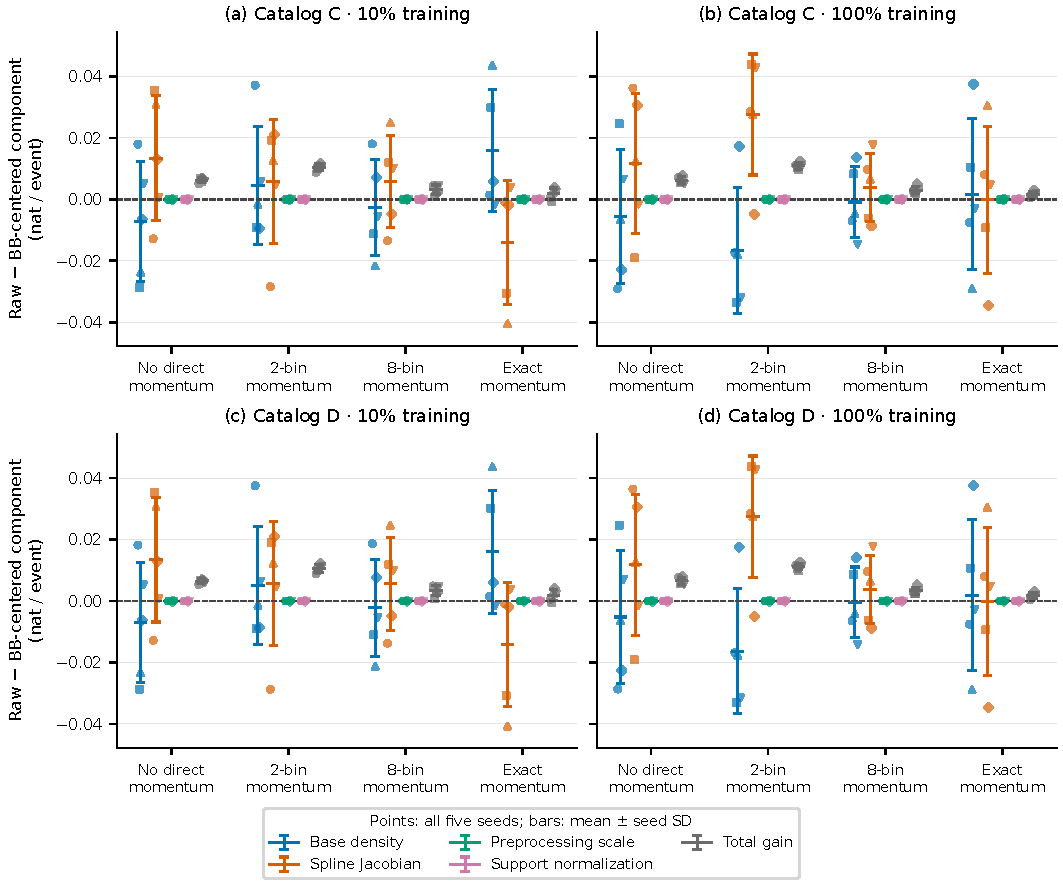
\includegraphics[width=0.92\linewidth]{information_exact_density_terms.pdf}
\caption{Additive contributions to original-unit NLL gains. The total is
shown alongside the four components and is not an additional contribution.
Bars show optimizer-seed SD. Support corrections are included even when
their float32 values are zero.}
\label{fig:supp_density_terms}
\end{figure}

Operational residual summaries include means and medians, standard deviations,
interquartile ranges, quantile asymmetry and tail widths. Predictive CDF
diagnostics include the fraction below the predicted median and the fraction
inside the predictive interquartile interval, each with nominal value $0.5$.
They use normalized predictive CDFs with stable log-CDF and log-survival
expressions. All are descriptive; pooling within a physical group can hide
finer conditional errors.

\subsection{Location burden under information refinement}
All expectations below refer to the eligible population $S=1$. Let
$V=\pin$, $W=(t,q)$, $m(V,W)=\mathbb E[Y\mid V,W]$, and let the
deterministic center $c(V,W)$ and $Y$ have finite second moments. The total
variance identity separates intrinsic complete-condition variation from
unobserved-momentum location variation:
\begin{equation}
 \operatorname{Var}(Y-c\mid W)=
 \mathbb E[\operatorname{Var}(Y\mid V,W)\mid W]
 +\operatorname{Var}_V(m-c\mid W).
\end{equation}
For illustration, consider a residual
Gaussian family with a freely fitted measurable mean $\mu(W)$ and the same
positive fixed variance $\sigma^2$ in both representations. Assuming finite
second moments under the same data distribution, and omitting support
truncation, its minimum expected NLL
relative to the corresponding Raw family differs by
\begin{equation}
 \mathcal L_c^*-\mathcal L_{\raw}^*
 =\frac{\mathbb E_W\!\left[
 \operatorname{Var}_V(m-c\mid W)-\operatorname{Var}_V(m\mid W)
 \right]}{2\sigma^2}.
 \label{eq:gaussian_illustration}
\end{equation}
This restricted-family example permits either direction of benefit. It is not
a performance formula for the trained spline flows.

The same distinction applies to partial information. For a measurable
coarsening $H(V)$, let $\mathcal G_H=\sigma(W,H(V))$ and define
$B_c(H)=\mathbb E[\operatorname{Var}(m-c\mid\mathcal G_H)]$, with
$B_{\raw}=B_0$. Assume finite second moments for $Y$ and the deterministic
measurable center $c$ in the eligible population. For nested information
$\mathcal G_{H_1}\subseteq\mathcal G_{H_2}$,
\begin{equation}
 B_c(H_1)-B_c(H_2)=\mathbb E\!\left[
 \left\{\mathbb E[m-c\mid\mathcal G_{H_2}]
       -\mathbb E[m-c\mid\mathcal G_{H_1}]\right\}^{2}\right]\geq0.
 \label{eq:information_refinement}
\end{equation}
Each location burden therefore decreases or stays fixed as information is
refined, but their difference $B_{\raw}(H)-B_c(H)$ need not be monotone.
In an abstract four-state example, take $W$ constant and let $A$ and $B$ be independent symmetric variables taking values
$-1$ and $+1$, let $V=2A+B$, and set $m=A$ and $c=A-B$. With no information,
with $A$ observed, and with $V$ observed, the difference is $0,-1,0$.
Under exact $V$, both location burdens vanish. The difference is proportional
to the representation gain in the fixed-variance Gaussian illustration;
these population identities do not imply monotonic NLL improvement for the
trained spline flows.

A translation does not alter the true variance at fixed complete conditions:
$\operatorname{Var}(Y-c\mid V,W)=\operatorname{Var}(Y\mid V,W)$.
Dependence of scale or shape on $V$ can remain in the residual distribution
even when the center matches its mean well. The location identity consequently
motivates a diagnostic, not a unique decomposition of likelihood gains into
location, scale and shape causes. General incompatibility between a prescribed
representation and unavailable neural information remains a theoretical
possibility; the empirical comparisons in the main article establish their measured
effects in the stated setting.



The empirical source diagnostic uses the reserved 298,939-row source
diagnostic partition. Within each thickness--charge stratum, 56 momentum
bins refine the two- and eight-bin neural encodings and the seven reporting
bins. The event-weighted variance of fine-bin residual means around their
information-cell mean approximates the remaining location burden. The main
figure shows its square root. The original-unit panel uses the saved 100\%
preprocessing record once; fraction-specific standardized panels use their
respective scales. Subtracting a fitted constant does not change population
location variance; tiny floating-point differences between the two saved
original-unit summaries are documented in the figure provenance record.

\section{Fitted-center, capacity and training-fraction comparisons}
\label{sec:secondary}

The secondary matrix uses exact momentum, four representations, two capacities,
three fractions and five paired seeds. Its 23 contrasts per catalog comprise
18 representation comparisons and five differences of centering gains across
capacities or fractions. Fitted centers use training data only and remain
fixed during flow fitting. All seed exceptions are retained; the spreads
describe optimizer variability rather than event-bootstrap uncertainty.

\begingroup
\small
\setlength{\tabcolsep}{3pt}
\begin{longtable}{lllrrr}
\caption{Complete secondary center, capacity and training-fraction contrasts on fresh catalog C, all with exact momentum inputs. $R$, $B$, $L$ and $P$ denote Raw, BB-centered, Linear center and Polynomial-ridge center. $D(A,B)=\mathrm{NLL}(A)-\mathrm{NLL}(B)$, so positive values favor the second model. Small and Large have widths 32 and 128. $\Delta=D(R,B)$; the final five rows compare this gain across capacities or fractions, not absolute NLL. Effects are in units of 0.001 nat per eligible event. Means, sample SDs, ranges and positive/negative/zero counts use five paired optimizer seeds. These descriptive seed spreads are not event-bootstrap intervals. Catalogs C and D are reported separately.}\label{tab:editorial-secondary-current-C}\\
\toprule Contrast & Capacity & Train (\%) & Mean (SD) & Seed range & $+/-/0$\\ \midrule \endfirsthead
\toprule Contrast & Capacity & Train (\%) & Mean (SD) & Seed range & $+/-/0$\\ \midrule \endhead
$D(R,B)$ & Small & 10 & +1.845 (1.855) & [-0.619, +3.899] & 4/1/0\\
$D(P,B)$ & Small & 10 & +2.410 (0.887) & [+1.453, +3.740] & 5/0/0\\
$D(L,R)$ & Small & 10 & -0.898 (1.669) & [-3.777, +0.454] & 2/3/0\\
\midrule
$D(R,B)$ & Large & 10 & +1.790 (1.524) & [+0.355, +4.266] & 5/0/0\\
$D(P,B)$ & Large & 10 & +3.234 (1.139) & [+1.557, +4.331] & 5/0/0\\
$D(L,R)$ & Large & 10 & -1.088 (2.265) & [-4.135, +1.964] & 1/4/0\\
\midrule
$D(R,B)$ & Small & 30 & +1.398 (0.908) & [+0.446, +2.774] & 5/0/0\\
$D(P,B)$ & Small & 30 & +1.105 (0.819) & [+0.416, +2.203] & 5/0/0\\
$D(L,R)$ & Small & 30 & -0.839 (0.500) & [-1.564, -0.256] & 0/5/0\\
\midrule
$D(R,B)$ & Large & 30 & +1.907 (1.425) & [+0.587, +4.292] & 5/0/0\\
$D(P,B)$ & Large & 30 & +2.725 (1.285) & [+1.569, +4.567] & 5/0/0\\
$D(L,R)$ & Large & 30 & -1.199 (0.705) & [-2.375, -0.470] & 0/5/0\\
\midrule
$D(R,B)$ & Small & 100 & +1.550 (0.923) & [+0.491, +2.979] & 5/0/0\\
$D(P,B)$ & Small & 100 & +1.681 (0.626) & [+1.089, +2.747] & 5/0/0\\
$D(L,R)$ & Small & 100 & -0.881 (1.112) & [-1.961, +0.376] & 2/3/0\\
\midrule
$D(R,B)$ & Large & 100 & +2.264 (1.534) & [+0.562, +4.135] & 5/0/0\\
$D(P,B)$ & Large & 100 & +2.233 (2.011) & [-0.730, +4.339] & 4/1/0\\
$D(L,R)$ & Large & 100 & -1.136 (1.359) & [-3.538, -0.259] & 0/5/0\\
\midrule
$\Delta_{32}-\Delta_{128}$ & Small--Large & 10 & +0.055 (1.812) & [-1.946, +1.897] & 3/2/0\\
$\Delta_{32}-\Delta_{128}$ & Small--Large & 30 & -0.509 (1.758) & [-2.509, +2.188] & 2/3/0\\
$\Delta_{32}-\Delta_{128}$ & Small--Large & 100 & -0.714 (1.417) & [-2.788, +1.209] & 1/4/0\\
\midrule
$\Delta_{10}-\Delta_{100}$ & Small & 10--100 & +0.295 (1.313) & [-1.778, +1.739] & 4/1/0\\
$\Delta_{10}-\Delta_{100}$ & Large & 10--100 & -0.474 (2.488) & [-2.947, +3.704] & 1/4/0\\
\bottomrule
\end{longtable}
\endgroup

\clearpage
\begingroup
\small
\setlength{\tabcolsep}{3pt}
\begin{longtable}{lllrrr}
\caption{Complete secondary center, capacity and training-fraction contrasts on fresh catalog D, all with exact momentum inputs. $R$, $B$, $L$ and $P$ denote Raw, BB-centered, Linear center and Polynomial-ridge center. $D(A,B)=\mathrm{NLL}(A)-\mathrm{NLL}(B)$, so positive values favor the second model. Small and Large have widths 32 and 128. $\Delta=D(R,B)$; the final five rows compare this gain across capacities or fractions, not absolute NLL. Effects are in units of 0.001 nat per eligible event. Means, sample SDs, ranges and positive/negative/zero counts use five paired optimizer seeds. These descriptive seed spreads are not event-bootstrap intervals. Catalogs C and D are reported separately.}\label{tab:editorial-secondary-current-D}\\
\toprule Contrast & Capacity & Train (\%) & Mean (SD) & Seed range & $+/-/0$\\ \midrule \endfirsthead
\toprule Contrast & Capacity & Train (\%) & Mean (SD) & Seed range & $+/-/0$\\ \midrule \endhead
$D(R,B)$ & Small & 10 & +1.876 (1.836) & [-0.491, +4.072] & 4/1/0\\
$D(P,B)$ & Small & 10 & +2.381 (0.891) & [+1.465, +3.677] & 5/0/0\\
$D(L,R)$ & Small & 10 & -0.715 (1.750) & [-3.726, +0.671] & 2/3/0\\
\midrule
$D(R,B)$ & Large & 10 & +1.902 (1.481) & [+0.496, +4.325] & 5/0/0\\
$D(P,B)$ & Large & 10 & +3.102 (1.220) & [+1.338, +4.415] & 5/0/0\\
$D(L,R)$ & Large & 10 & -1.062 (2.089) & [-3.974, +1.692] & 1/4/0\\
\midrule
$D(R,B)$ & Small & 30 & +1.543 (0.950) & [+0.511, +2.951] & 5/0/0\\
$D(P,B)$ & Small & 30 & +1.253 (0.728) & [+0.463, +2.164] & 5/0/0\\
$D(L,R)$ & Small & 30 & -0.630 (0.545) & [-1.384, -0.012] & 0/5/0\\
\midrule
$D(R,B)$ & Large & 30 & +2.143 (1.377) & [+0.757, +4.422] & 5/0/0\\
$D(P,B)$ & Large & 30 & +2.965 (1.086) & [+2.140, +4.520] & 5/0/0\\
$D(L,R)$ & Large & 30 & -1.124 (0.709) & [-2.281, -0.416] & 0/5/0\\
\midrule
$D(R,B)$ & Small & 100 & +1.659 (0.973) & [+0.371, +3.059] & 5/0/0\\
$D(P,B)$ & Small & 100 & +1.911 (0.688) & [+1.255, +3.059] & 5/0/0\\
$D(L,R)$ & Small & 100 & -0.737 (1.113) & [-2.055, +0.480] & 2/3/0\\
\midrule
$D(R,B)$ & Large & 100 & +2.348 (1.704) & [+0.413, +4.514] & 5/0/0\\
$D(P,B)$ & Large & 100 & +2.389 (2.208) & [-0.874, +4.762] & 4/1/0\\
$D(L,R)$ & Large & 100 & -1.130 (1.364) & [-3.556, -0.340] & 0/5/0\\
\midrule
$\Delta_{32}-\Delta_{128}$ & Small--Large & 10 & -0.027 (1.745) & [-2.059, +2.076] & 3/2/0\\
$\Delta_{32}-\Delta_{128}$ & Small--Large & 30 & -0.600 (1.750) & [-2.424, +2.194] & 1/4/0\\
$\Delta_{32}-\Delta_{128}$ & Small--Large & 100 & -0.689 (1.537) & [-2.858, +1.479] & 1/4/0\\
\midrule
$\Delta_{10}-\Delta_{100}$ & Small & 10--100 & +0.216 (1.221) & [-1.811, +1.310] & 4/1/0\\
$\Delta_{10}-\Delta_{100}$ & Large & 10--100 & -0.446 (2.565) & [-2.781, +3.912] & 1/4/0\\
\bottomrule
\end{longtable}
\endgroup


\clearpage
\section{Numerical implementation and reproducibility}
\label{sec:numerical_boundary}

\begin{table}[!htbp]
\centering
\caption{Precision roles in the frozen implementation. Float64 reductions
do not restore precision lost during model evaluation.}
\label{tab:supp_precision}
\begin{tabular}{p{0.68\linewidth}l}
\toprule Stage & Arithmetic \\
\midrule
Physical-center evaluation and preprocessing fit & float64 \\
Applied standardization ($z$ and $b$) & float32 \\
Neural inputs, parameters, inference and optimizer & float32 \\
Validation mean used to select checkpoints & float32 \\
Saved per-event log scores & float32 \\
Paired subtraction, means and bootstrap reductions & float64 \\
\bottomrule
\end{tabular}
\end{table}

The center and fitted $\mu,s$ are computed in float64 (Table~\ref{tab:supp_precision}). Before neural
evaluation, $Y$, $c$, $\pin$ and $s$ are separately converted to float32;
the subsequent subtraction and division defining $z$ and $b$, including
application of $\mu$, use float32 arithmetic. Selecting a checkpoint with
a different precision for the validation reduction would change the frozen
training procedure.

The density uses stable log-sigmoid and softplus expressions. In base-flow
coordinates $a$ and $b$ for an event and its upper support bound, the truncated
log-survival expression is
\begin{equation}
 \log S=-\operatorname{softplus}(a)+\log[-\operatorname{expm1}(a-b)].
\end{equation}
This avoids directly subtracting two CDFs close to one. At the exact upper
boundary, log density and log survival are $-\infty$ and log CDF is zero.
The scorer rejects nonfinite density/decomposition values; legitimate
infinite log-tail probabilities are handled separately.

Three existing mathematical regression tests passed. Additional deterministic
checks used 18 tail cases per dtype, base support bounds from $-1000$ to
$1000$, and distances including one representable ULP below the boundary.
An untrained fixed flow in its identity tails was compared with a 100-digit
Decimal reference. In these synthetic checks, no events were generated or read,
no saved checkpoint was evaluated, and no training was performed. Maximum
observed absolute errors are listed in Table~\ref{tab:supp_synthetic_errors}.

\begin{table}[!htbp]
\centering
\caption{Maximum observed absolute errors in synthetic identity-tail checks
against a 100-digit Decimal reference across 18 tail cases per dtype.}
\label{tab:supp_synthetic_errors}
\begin{tabular}{lrrrr}
\toprule
Dtype & Log density & Log CDF & Log survival & $|\mathrm{CDF}+\mathrm{SF}-1|$\\
\midrule
float32 & $9.14\times10^{-9}$ & $1.30\times10^{-9}$ & $1.05\times10^{-5}$ & $0$\\
float64 & $2.58\times10^{-15}$ & $2.04\times10^{-9}$ & $7.11\times10^{-15}$ & $2.02\times10^{-9}$\\
\bottomrule
\end{tabular}
\end{table}

The float64 log-CDF discrepancy reflects the default softplus linear
approximation above its threshold of 20; it is not evidence of uniform
$10^{-12}$ accuracy. Tested boundary values and log-survival gradients were
correct and finite where required. These checks are not a worst-case error
bound over every learned spline parameterization or device.

Input resolution is a separate limit. At momentum 0.3, 0.65 and 1.0 GeV/$c$,
an input only one float64 ULP inside the upper support becomes equal to the
bound after float32 conversion. This establishes a rounding possibility.
The follow-up audit below measures its incidence in the complete formal C/D
samples without modifying those samples or rerunning the density models.

\subsection{Complete event coverage and input margins}

This follow-up audit was performed after the C/D results were known. All
500,000 launched ledger records in each catalog were read. Eligibility was
reconstructed from the saved first-visit entry/exit geometry and exit momentum,
without retracing Geant4 steps. The resulting 499,285 C and 499,275 D eligible
rows matched every saved scoring input, including event identifiers and their
order. The 715 and 725 ineligible events were excluded by the physical event
contract before scoring, not by numerical filtering. The saved target agreed
bitwise with the independently recomputed $Y=p_{\rm in}-p_{\rm out}$.

For each eligible row, define
\begin{equation}
 m_{32}=\operatorname{fl}_{32}\!\left(
 \operatorname{fl}_{32}(p_{\rm in})-\operatorname{fl}_{32}(Y)\right).
\end{equation}
Both catalogs have zero nonfinite, zero and negative margins. None has a
positive margin at or below $10^{-3}$ GeV/$c$, or at or below 1024 downward
ULPs at $p_{\rm in}^{(32)}$; the smallest margin-to-ULP ratios are
$8.2840175\times10^6$ and $8.311172\times10^6$, respectively. The cumulative
thresholds were fixed before the ledger scan. Here one downward ULP is
$p^{(32)}-\operatorname{nextafter}(p^{(32)},-\infty)$.
Table~\ref{tab:actual_support_margins} reports the distribution after computing
the subtraction in float32 and promoting its result to float64 for linear
quantile interpolation. A float64 difference of two rounded inputs is a
distinct diagnostic, retained separately in the audit records.

\begin{table}[!htbp]
\centering\small
\setlength{\tabcolsep}{4pt}
\caption{Actual float32 support-margin distributions, in GeV/$c$. Counts
include all eligible events. Zero, negative and nonfinite counts are zero in
both catalogs. The complete finer quantiles and seven momentum-bin summaries
are retained with the aggregate audit.}
\label{tab:actual_support_margins}
\begin{tabular}{lrrrrrr}
\toprule
Catalog & Events & Minimum & 1\% & Median & 99\% & Maximum\\
\midrule
C & 499,285 & 0.295779943 & 0.306910386 & 0.649518907 & 0.992840517 & 0.999970257\\
D & 499,275 & 0.297881365 & 0.306801179 & 0.650127709 & 0.992949682 & 0.999970496\\
\bottomrule
\end{tabular}
\end{table}

All 240 registered models per catalog retained the complete eligible-event
count and event-order digest. Recomputing only their frozen centers and
standardization, without evaluating a neural flow, reproduced all 960 saved
$z$ and $b$ arrays bitwise: 479,308,800 values, with no mismatch. The smallest
$b-z$ was 751.749807, and no saved $z$ reached or exceeded $b$.
All 5280 saved model-component arrays passed their recorded byte, shape and
dtype checks, and all event log densities were finite. Together these checks
show that no eligible row was silently dropped or numerically rejected from
the completed scores. They are a ledger and preprocessing reconciliation,
not a new neural-density evaluation or a validation of the transport physics.

\subsection{Actual support log-CDFs and their mathematical scale}

Across all 480 registered model--catalog evaluations, every saved support
log-CDF is float32 negative zero: 239,654,400 entries, zero nonzero values and
zero nonfinite values. Thus all its recorded quantiles are zero. These are
repeated model--event evaluations, not that many independent events; the 20
Full rerun pairs per catalog retain their exact duplicate identities.
Table~\ref{tab:actual_support_bounds} separates the primary 80 runs from the
160 earlier registered runs.

\begin{table}[!htbp]
\centering\small
\caption{Range of recorded standardized support bounds across every eligible
event and model in each cohort. Each model has bound 8 for both spline layers.
All support log-CDF entries are negative zero; all saved $z<b$.}
\label{tab:actual_support_bounds}
\begin{tabular}{llrrr}
\toprule
Catalog & Cohort & Model--event entries & Minimum $b$ & Maximum $b$\\
\midrule
C & Primary 80 & 39,942,800 & 761.355408 & 2776.529053\\
C & Earlier 160 & 79,885,600 & 761.350159 & 2776.529053\\
D & Primary 80 & 39,942,000 & 761.354797 & 2776.541260\\
D & Earlier 160 & 79,884,000 & 761.349548 & 2776.543945\\
\bottomrule
\end{tabular}
\end{table}

The zeros have a quantitative explanation. Every saved bound exceeds 761.349,
well outside the spline interval $[-8,8]$. Each layer is exactly the identity
there, so its transformed base bound equals $b$, independently of the neural
conditioner outputs. With the standard logistic base,
\begin{equation}
 \epsilon(b)=1-F_\theta(b\mid h)=\frac{1}{1+e^b},\qquad
 \eta(b)=-\log F_\theta(b\mid h)=\log(1+e^{-b}).
\end{equation}
For $b>0$, both satisfy $0<\epsilon(b),\eta(b)<e^{-b}$. The smallest recorded
bound therefore gives $\epsilon,\eta<10^{-330}$ for every evaluated entry.
The excluded probability mass and the likelihood normalization correction
are mathematically positive, but are smaller than half the smallest positive
float64 subnormal number. A float64 re-expression would also round them to
zero; it would not reveal a representable nonzero distribution. The aggregate
audit retains the $b$ quantiles and log-domain bounds, rather than assigning
artificial nonzero probabilities.

This certificate concerns the mathematical logistic function evaluated at the
saved rounded bounds. It uses the verified identity-tail construction and
does not rerun the neural networks in float64. It explains why normalization
has no observable contribution for these models and catalogs; the term remains
in the likelihood and is not assumed negligible for other models or inputs.


\subsection{Reproducibility and evidence identities}
All 80 primary checkpoints passed complete source-validation replay before
fresh generation. A separate saved-output audit reaggregated all 480 registered
model--catalog scores, the 16 primary and 336 local estimates per catalog,
and the 2000 paired bootstrap draws. The source-validation comparison is
descriptive because those events selected the checkpoints; its original
complete table is preserved in the standalone historical/presentation archive.

For inventory reconciliation, the frozen scoring registry contains 240 run
records: 80 primary executions and 160 previously fitted runs. The latter
union comprises a 60-run comparison and a 120-entry capacity/fraction matrix
sharing 20 entries. Twenty exact-momentum primary executions reproduce
earlier Small exact-conditioner state tensors and source/C/D log scores
exactly. They are overlapping predictors, not independent replications.
The secondary table file preserves all 41 contrasts per catalog in two parts:
23 current fitted-center/capacity contrasts here, and 18 older-design/control
contrasts in the historical archive. No scientific result is removed from
the retained records by this presentation split.

The companion GitHub repository (\url{https://github.com/xschang1002/EPJC},
release tag \texttt{v1.0.0-epjc}) distinguishes three reproduction levels.
Its lightweight Git source tree omits binary model checkpoints for direct
version-control portability while retaining all 240 run manifests and
cryptographic checkpoint SHA-256 digests (with binary checkpoints optionally
verified when supplied via a companion archive via \texttt{-{}-checkpoint-root}).
Using the documented software dependencies, the single entry point
\texttt{python reproduce.py} reconstructs all tables, all 21 figures, the
saved-draw bootstrap intervals, the five-seed sensitivity CSVs, and the four
C/D predictive and residual diagnostic summaries without requiring the original
local filesystem paths.

Event-level replay additionally requires the original event ledgers,
preprocessing inputs and per-event scores. Complete regeneration requires
those inputs, the Geant4 environment, model-training dependencies and the
frozen sampling and training protocols. These latter two levels cannot be
performed from the aggregate repository alone; raw event ledgers and
per-event score arrays are retained in local archival storage verified by the
published SHA-256 manifests and are available from the corresponding author
upon reasonable request.

\subsection{Display names and immutable run identifiers}
\label{sec:display_mapping}
The presentation uses descriptive display terminology while model files,
frozen code, run identifiers, protocols and hashes retain their original
names (Table~\ref{tab:editorial-display-names}).
\begin{table}[!htbp]
\centering\small
\caption{Paper display names and frozen implementation identifiers. Display names do not change saved models or protocol definitions.}
\label{tab:editorial-display-names}
\begin{tabular}{lll}
\toprule Paper display name & Table symbol & Frozen identifier\\
\midrule
No direct momentum & $N$ & Hidden5\\
2-bin momentum & $M_2$ & Coarse2\\
8-bin momentum & $M_8$ & Coarse8\\
Exact momentum & $E$ & Full5\\
Raw & $R$ & Raw\\
BB-centered & $B$ & CorrectedPhysics\\
Linear center & $L$ & Simple\\
Polynomial-ridge center & $P$ & Learned\\
\bottomrule
\end{tabular}
\end{table}


\section{Brief development history}
A unit-conversion error in a preliminary center was corrected before the
primary study. The affected preliminary results are excluded from the present
conclusions; development records and earlier exploratory analyses are retained
in the repository archive (\texttt{historical\_archive\_20261108}).

\end{document}
